% *********************************************************************
% © 2021–2024 Jeremy Sylvestre
%
% Permission is granted to copy, distribute and/or modify this document
% under the terms of the GNU Free Documentation License, Version 1.3 or
% any later version published by the Free Software Foundation; with no
% Invariant Sections, no Front-Cover Texts, and no Back-Cover Texts. A
% copy of the license is included in the appendix entitled “GNU Free
% Documentation License” that appears in the output document of this
% PreTeXt source code. All trademarks™ are the registered® marks of
% their respective owners.
%
% *********************************************************************

\newcommand*{\xmin}{-2}
\newcommand*{\xmax}{2}
\newcommand*{\ymin}{-2}
\newcommand*{\ymax}{2}

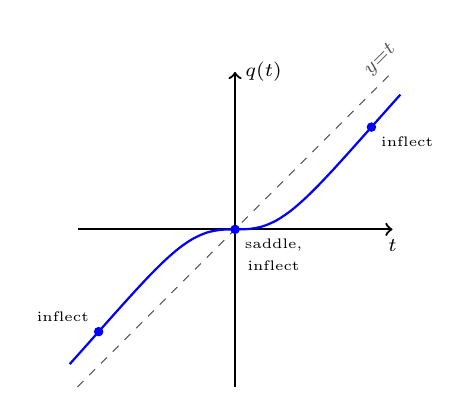
\begin{tikzpicture}
[
	closedpt/.style={circle,draw,fill,inner sep=0pt,minimum size=3pt},
	openpt/.style={circle,draw,inner sep=0pt,minimum size=3pt}
]

	\draw[dashed,black!66!white] (\xmin,\ymin) -- node[above,sloped,at end] {$\scriptstyle y = t$} (\xmax,\ymax);

	% axes
	\draw[->,thick] (\xmin,0) -- (\xmax,0) node[below] {$\scriptstyle t$};
	\draw[->,thick] (0,\ymin) -- (0,\ymax) node[right] {$\scriptstyle q(t)$};

	\draw[blue,thick,domain=-2.1:2.1,smooth] plot (\x,{\x * \x * \x / (\x * \x + 1)});

	\node[blue,closedpt] at (1.732,1.299) {};
	\node[below right] at (1.732,1.299) {\tiny inflect};
	\node[blue,closedpt] at (-1.732,-1.299) {};
	\node[above left] at (-1.732,-1.299) {\tiny inflect};
	\node[blue,closedpt] at (0,0) {};
	\node[below right, align=center] at (0,0) {\tiny saddle, \\[-4pt] \tiny inflect};

\end{tikzpicture}
